% https://tex.stackexchange.com/a/765260
\documentclass[tikz,border=5pt]{standalone}
\usepackage{newtx}
\begin{document}
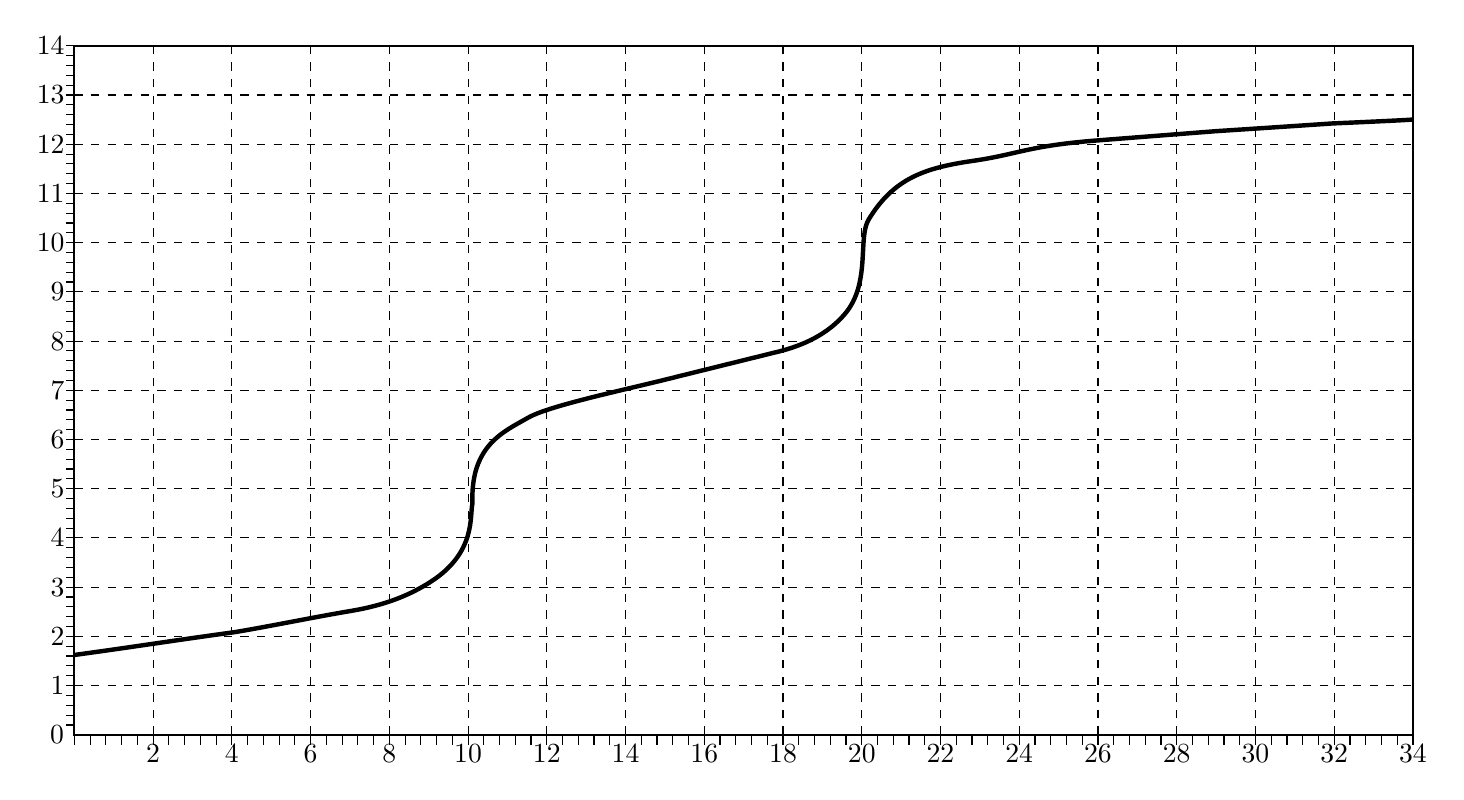
\begin{tikzpicture}[yscale=1.25]
\draw[ultra thick] (0,0.811)
.. controls (0.692,0.886) and (1.354,0.969) .. (2.039,1.043)
.. controls (2.526,1.109) and (3.029,1.193) .. (3.517,1.259)
.. controls (3.962,1.319) and (4.276,1.425) .. (4.532,1.558)
.. controls (5.104,1.854) and (5.019,2.226) .. (5.056,2.351)
.. controls (5.028,2.94) and (5.451,3.079) .. (5.766,3.223)
.. controls (6.04,3.348) and (7.033,3.511) .. (7.678,3.643)
.. controls (8.099,3.726) and (8.521,3.81) .. (8.942,3.893)
.. controls (9.258,3.956) and (9.565,4.068) .. (9.785,4.275)
.. controls (10.118,4.587) and (9.946,5.051) .. (10.088,5.236)
.. controls (10.406,5.653) and (10.799,5.76) .. (11.412,5.831)
.. controls (11.977,5.896) and (12.115,5.985) .. (12.998,6.039)
.. controls (13.494,6.07) and (13.99,6.101) .. (14.486,6.132)
.. controls (14.982,6.158) and (15.478,6.184) .. (15.974,6.211)
.. controls (16.457,6.228) and (16.94,6.246) .. (17,6.251);
\draw[thick] (0,0) node[left] {$0$} rectangle (17,7);
\foreach \x in {1,...,17} {
    \draw[dashed] (\x,0) node[below] {\inteval{2*\x}} -- (\x,7);
    \foreach \y in {0,.2,...,1} { \draw ({\x-\y},0) -- ++(0,-.1);}
}
\foreach \x in {.5,1,...,7} {
    \draw[dashed] (0,\x) node[left] {\fpeval{2*\x}} -- (17,\x);
    \foreach \y in {0,.1,...,.5} { \draw (0,{\x-\y}) -- ++(-.1,0);}
}
\end{tikzpicture}

\end{document}